\section{Estimating Link Travel Times and Correlations}
\label{sec:lttestimation} 

The prediction of an event is usually tainted with uncertainty. In the
case of the prediction of link travel times it is also generally not possible to
produce a prediction that is 100\% accurate, since there are too many
influencing factors like road condition, accidents, weather, time of the day,
day of the week or season. In contrast the methods we propose a
probabilistic prediction which includes all the effects that have been observed
before (historic data) and are influencing the traffic flow right now (current
data). For example if a street segment has often been the place of an accident
(e.g., every other day between 9.00am and 10.00am) then the historical data
will capture this effect and assign a high probability (e.g., 50\%) to the
prediction that the travel time on that segment will be higher than usual.
In this section we will develop three approaches to estimate probabilistic link
travel times and correlations between them.


\textbf{Probabilistic Link Travel Times: } There generally
exists two types of probabilistic link travel time representations
$c_{ij}^t$ of a link $(i,j)$, namely discrete and continuous models. 

% For the discrete representation the link travel time is discretized into into
% fixed time units ($\phi$) and each of these time units is associated with a probability. In the continuous case a parametrized function is used that
% represents the pdf over the link travel time. Common functions which are used in the continuous case are the
% normal distribution and the gamma distribution. Figure \ref{fig:models}
% illustrates the representation of a link travel time in the discrete case by a
% histogram and in the continuous case by a gamma distribution. To some extent, a
% discrete problem is more general because probability distributions from
% real-world applications are often available in discrete forms as probability
% mass functions . Also, any continuous probability function may be
% appropriately discretized as a pmf straightforwardly.

To represent the link travel time $c_{ij}^t$ with a continuous \textit{pdf}, a
suitable function is needed. Recent studies suggest that in road networks, the link
travel times are normally (e.g. \cite{Seshadri10}) or gamma
(e.g. \cite{Zockaei13}) distributed. To the best of our knowledge, no
approach exists, to compute the sum of several gamma distributed random
variables. Thus only approximate sampling approaches \cite{Zockaei13} or approaches discretizing the distributions \cite{Nie09b} have been proposed so far for the case where link travel times are assumed to be gamma distributed. In the first case, no extension for the time-dependent and correlated setting
exists and the latter case is covered by the discretized approach. For these
reasons we decided not to explicitly include the gamma distribution in the
present study. In the case of a normal distribution, the random variable
$c_{ij}^t$ is characterized by a mean $\mu_{ij}^t$ and a standard deviation $\sigma_{ij}^t$.

In the discrete case, the link travel time is represented by a discrete
probability mass function. For this the time domain has to be discretized.
The simplest discretization scheme, known as b-discrete, divides the time domain
$T = \{t | t = n\cdot \phi \wedge n \in \NN \}$ evenly into intervals of length $\phi$.
The corresponding probability mass function $F_{ij}$ of link travel time
$c_{ij}$ reads
\begin{equation}
	F_{ij}(b) = \begin{cases}\int_b^{b+\phi}f_{ij}(w)dw \qquad b =
	0,\phi,\ldots, (L-1)\phi\\
	\int_b^{\infty}f_{ij}(w)dw \qquad b =
	L \phi\\
	0 \qquad otherwise
	\end{cases} 
\end{equation}
where $L \phi$ is the maximal considered time horizon in the future.

Let us note that besides the b-discrete discretization scheme other schemes
\cite{Nie12} such as the $\alpha$-discrete scheme (where the support
is divided such that each interval has the same probability mass $\epsilon$) or
the adaptive discretization scheme (where starting from the b-discrete scheme,
intervals are consolidated until each interval has a minimum probability mass of
$1/L$) where proposed sacrificing some numerical accuracy.

\begin{figure*}
    \centering
    \subfigure[9:00am]{
        \label{fig:900}
        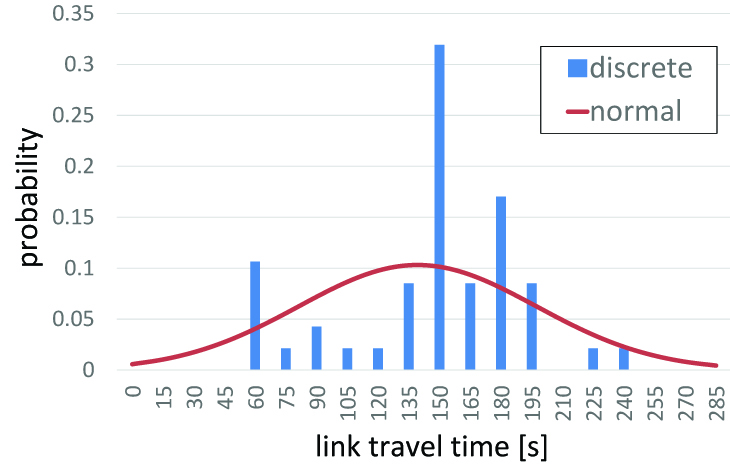
\includegraphics[width = 0.6\columnwidth]{figures/ltt_0900.jpg}
    }
    \subfigure[12:00pm]{
        \label{fig:1200}
        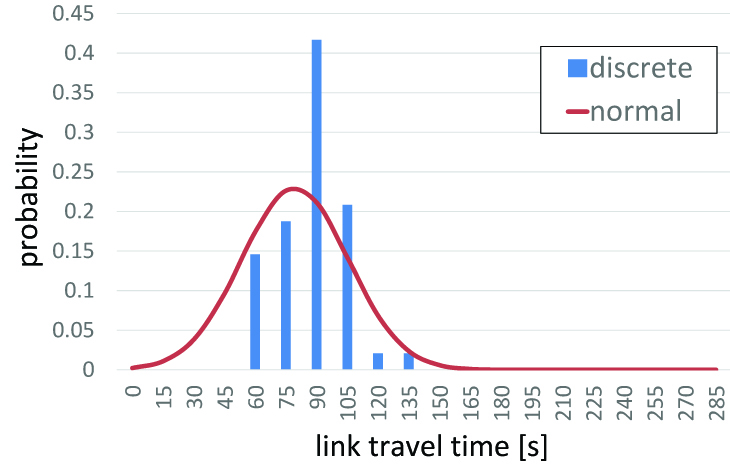
\includegraphics[width = 0.6\columnwidth]{figures/ltt_1200.jpg}
    }
    \subfigure[6:00pm]{
        \label{fig:1800}
        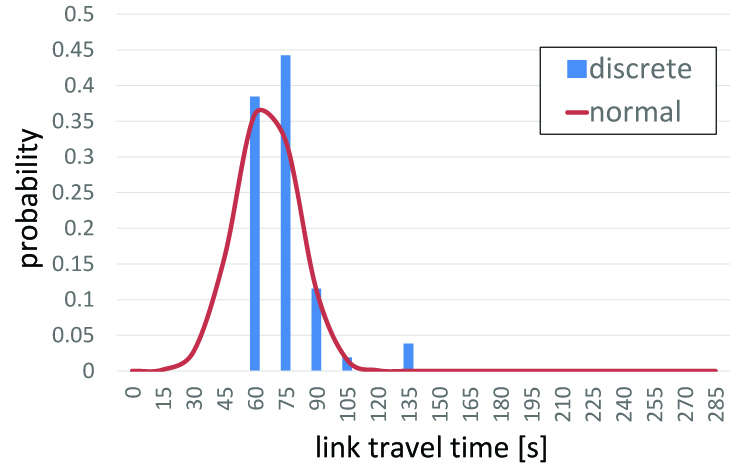
\includegraphics[width = 0.6\columnwidth]{figures/ltt_1800.jpg}
    }
    \caption{Historical model for a street segment for different times of a
    Monday}\label{fig:ltt}
\end{figure*}

\textbf{Correlations between Link Travel Times: } Even in the static case
(without time-dependent link travel times), the assumption that link travel times of two edges are independent from
each other is questionable in a real-world traffic network. Surely the
simplification of assuming independence helps on reducing resource allocation of many computations on these
networks. However, given a heavily congested link (resulting in a high
travel time), the adjacent link is usually also congested to a similar degree.
This simple observation illustrates that integrating some kind of correlation in
the model may yield a more exact representation of reality. Again we differentiate between the
discrete and the normally distributed case:

For the continuous case under the assumption of normal distributed link travel
times, we compute a correlation coefficient $\rho_{ij-kl}$ for the correlation
$corr(c_{ij},c_{kl})$ of any pair $((i,j), (k,l))$ of edges in the graph.

With the discrete case, we model correlation in the following manner. We assume
that link travel times may follow two different distributions depending on the condition of the link. A link may
either be non-congested (State-0) or congested (State-1) where each of these
two states is then associated with its own \textit{pmf}. The correlation between the states
of adjacent links are taken into account by introducing conditional
probabilities $\alpha^{uv}_{ij}$, meaning the probability of having link $(i,j)$
in state $v$, if the link leading to node $i$ is  in state $u$. This form of
correlation allows only for expressing correlation between adjacent links, but
is adopted by a variety of works, hence we follow this model. In the following
subsections, we will discuss our techniques to generate probabilistic link travel-times.  

% \begin{figure}
%     \centering
%     \subfigure[discrete pdf]{
%         \label{fig:discrete}
%         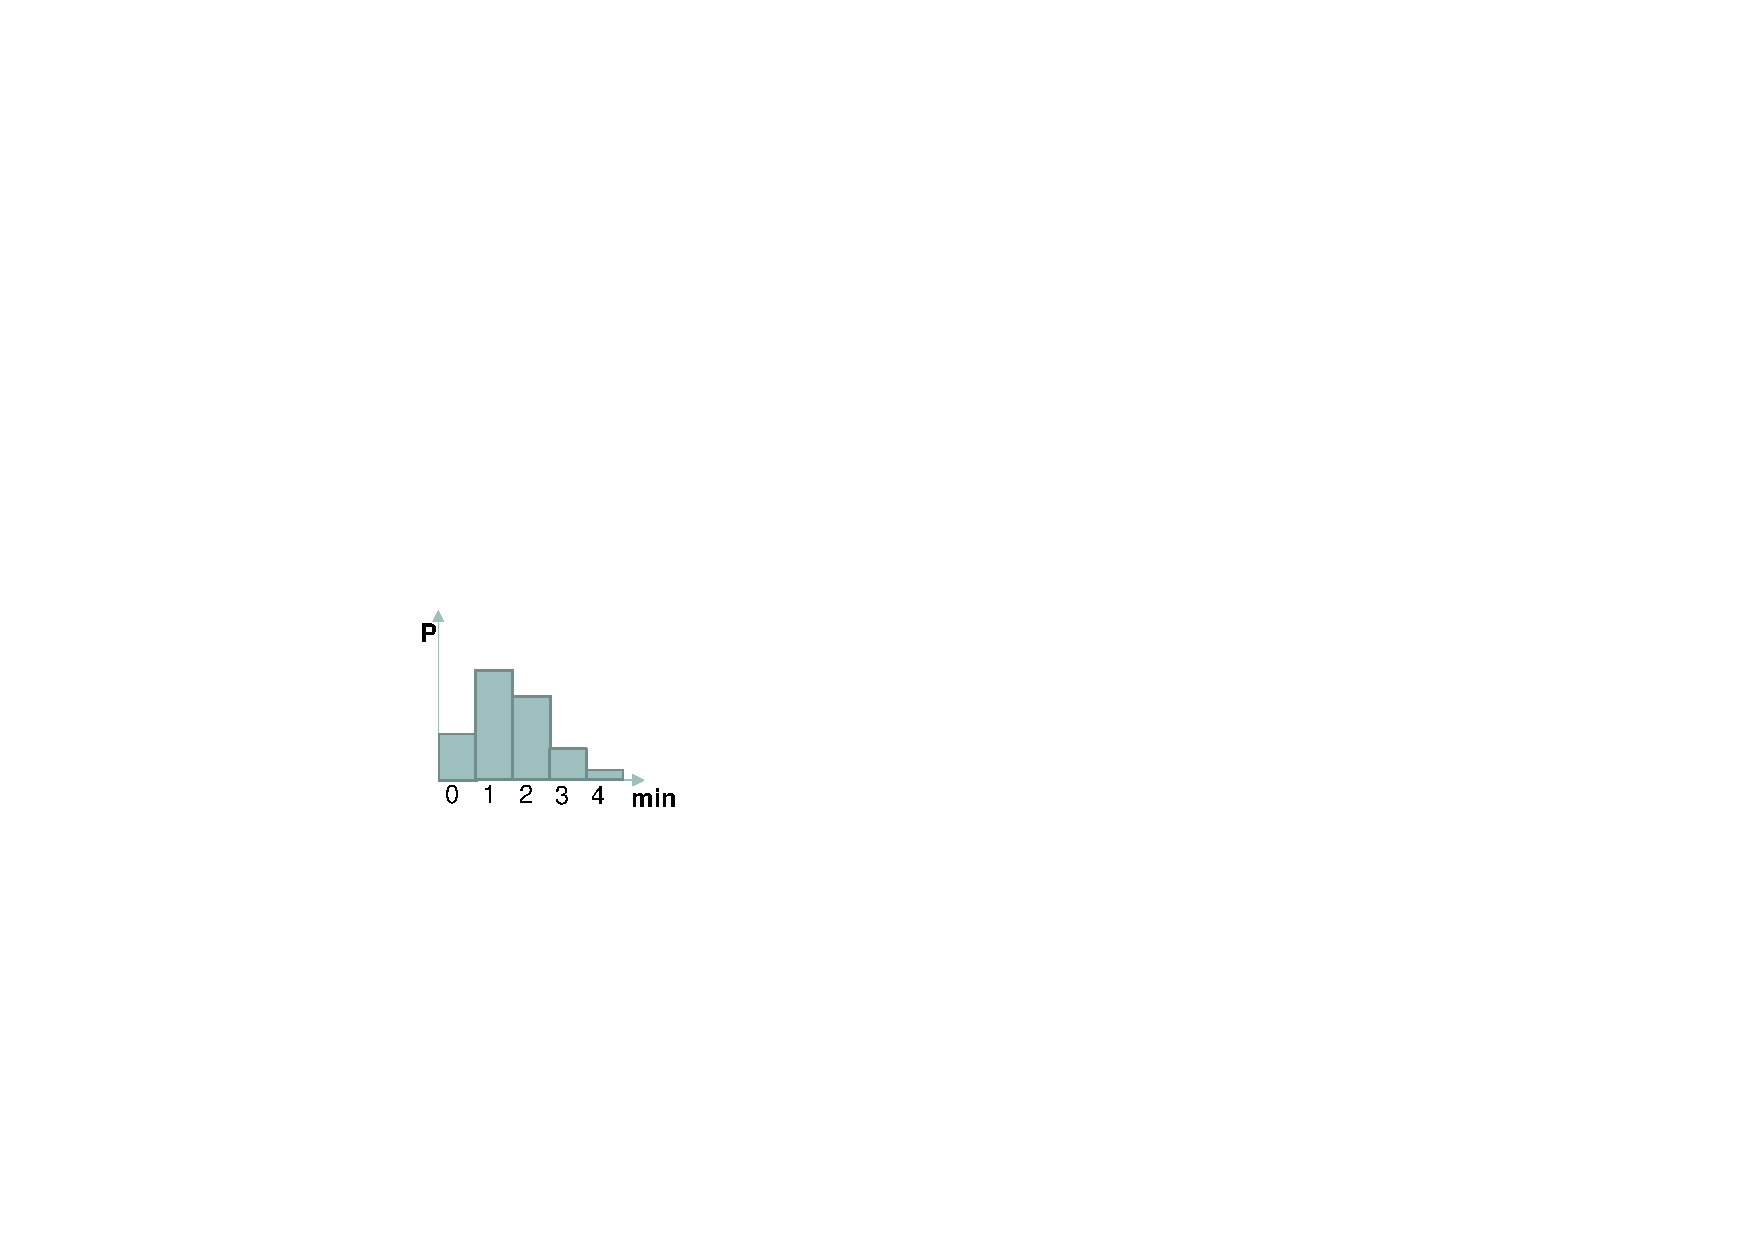
\includegraphics[width = 0.3\columnwidth]{figures/pdf_discrete.pdf}
%     }
%     \subfigure[continuous pdf]{
%         \label{fig:continuous}
%         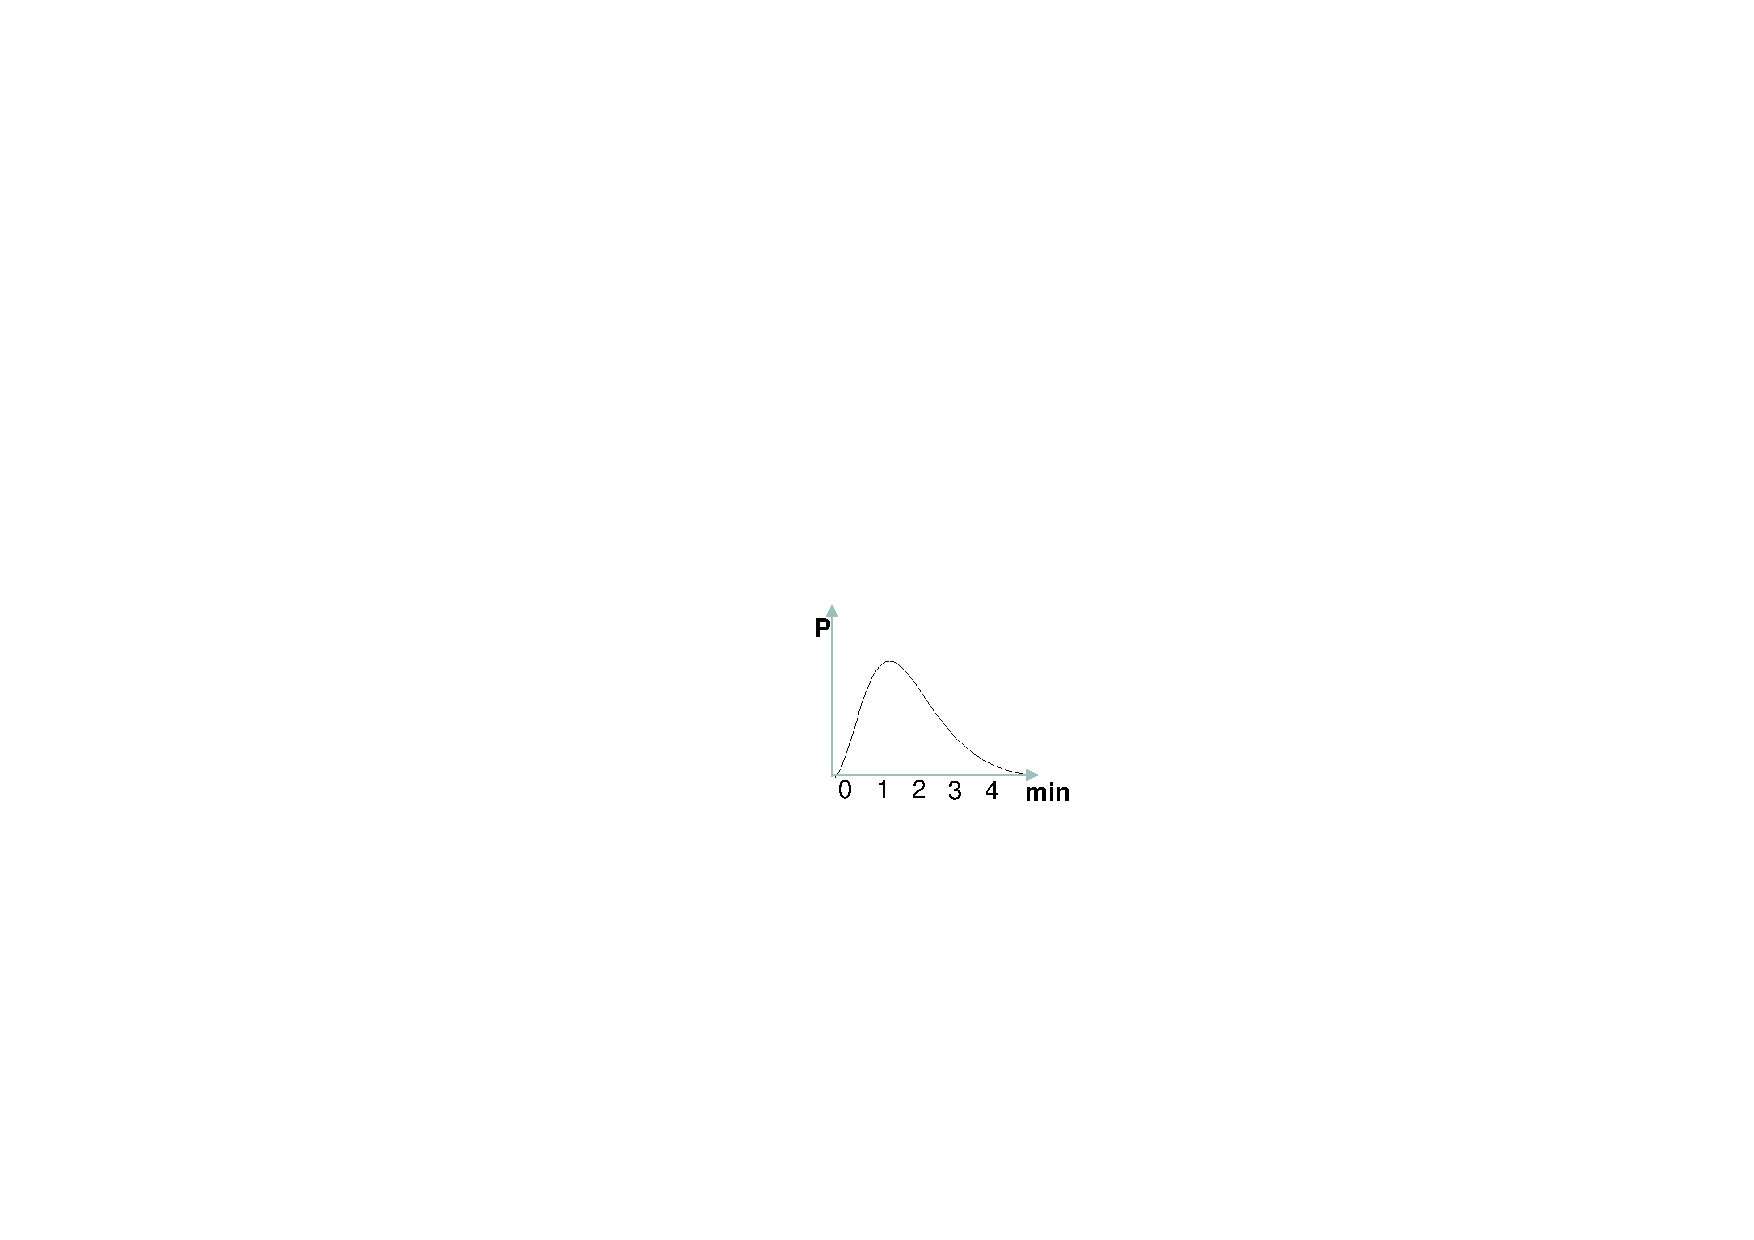
\includegraphics[width = 0.3\columnwidth]{figures/pdf_gamma.pdf}
%     }
%     \subfigure[ltt at rush hour]{
%         \label{fig:traffic}
%         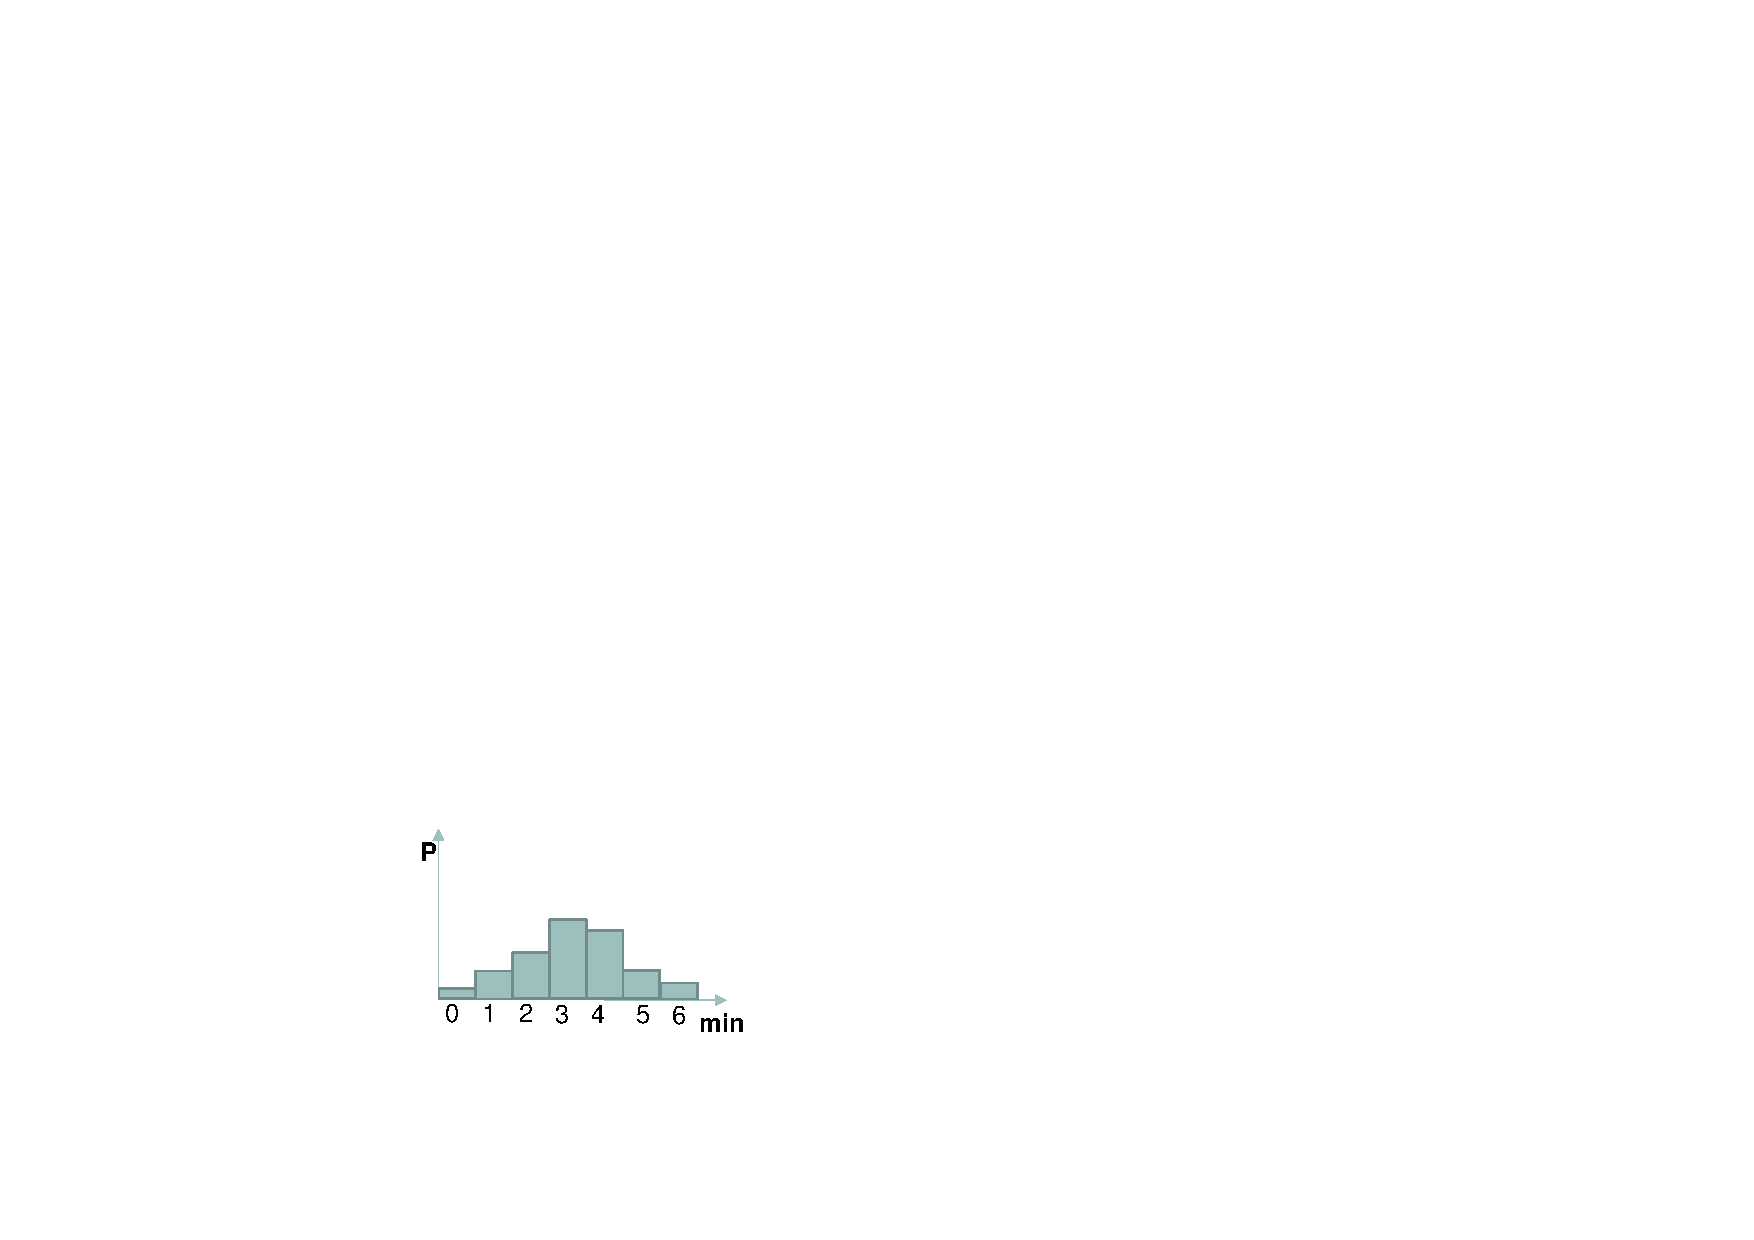
\includegraphics[width = 0.3\columnwidth]{figures/pdf_traffic.pdf}
%     }
%     \caption{Representation of link travel times}
%     \label{fig:models}
% \end{figure}

% The last section summarized existing works on reliable shortest-path search
% under the consideration of uncertainty of link travel times with a particular
% focus on the computation of the pdf representing the path travel time of a given
% path. However none of the mentioned works describes how to generally obtain the
% uncertain link travel times. Thus to the best of our knowledge there does
% neither exist an evaluation of the effectiveness of such approaches nor a
% comparison of several approaches with respect to the expected accuracy. We wish
% to close this research gap and provide methods how to obtain adequate uncertain
% link travel times and additional necessary parameters in order to provide
% meaningful outcomes. In the following we thus aim at obtaining a pdf (or pmf)
% representing $c_{ij}^t$ and parameters for describing the correlation
% $corr(c_{ij},c_{kl})$ between two edges $(i,j)$ and $(k,l)$.


% In order to allow for accurate parameter estimation we assume that the following
% data is present:
% \begin{itemize}
%   \item The graph of the road network to consider $G(V,E)$.
%   \item For each edge $(i,j) \in G$ in the network historical data about the
%   link travel time $c_{i,j}^t, t \in H = \{-A\phi, (-A+1)\phi, \ldots,
%   -\phi\}$.
%   \item For each edge $(i,j) \in G$ in the network the current link travel time
%   $c_{ij}^0$.
% \end{itemize}


\subsection{Prediction through Historical Data}
\label{subsec:historical}
To obtain a \textit{pdf} representing $c_{ij}^t$ for a future time $(t>0)$, a
simple approach is to use the available historical $h \in \{H| h < 0\}$ data and
summarize it.
Let us note that the link travel time $c_{ij}^h$ is not a random
variable but a certain value which is known. However, since using all available
historical data $c_{i,j}^h, \forall h \in H$ does not allow for
accurate probabilistic estimations. Rather a subset $H' \in H$ has to be chosen,
which resembles similar characteristics to the time $t$, for which the
prediction is made. For example, if we want to predict the behavior of edge
$(i,j)$ at 9:00am for the next Tuesday, an adequate set $H'$ might consist of
times $h$ which correspond to all Tuesdays 9:00am in the last year. The travel
time $c_{i,j}^h$ corresponding to last Tuesday 10:00pm might on the other hand
not be a good choice for the prediction. How to choose a set $H'$ is very
dependent on the characteristics of the underlying traffic network.
More details can be found in \cite{Pan12}.

For the continuous representation of the link travel time, we assume normal
distribution with the following parameters
\begin{gather}
	\mu_{ij}^t = \frac{1}{|H'|}\sum_{h\in H'} c_{i,j}^h\\ 
	(\sigma_{ij}^t)^2 = \frac{1}{|H'|}\sum_{h\in H'} (c_{ij}^h-\mu_{ij}^t)^2\\
	\rho_{ij-kl} = \frac{\sum_{h\in H} (c_{ij}^h - \mu_{ij}) (c_{kl}^h -
	\mu_{kl})}{(|H'-1| \sigma_{ij} \sigma_{kl})}
\end{gather}

For the case of discrete representation through a \textit{pmf} we set
\begin{gather}
F_{ij}^t(b) = \frac{1}{|H'|}\sum_{h\in H'} I(c_{ij}^h = b)
\end{gather}
where $I(c_{ij}^h = b)$ is an indicator variable which is 1 if $c_{ij}^h =
b$ and 0 otherwise. The \textit{pmf} of each edge is thus given by a histogram
assigning for each possible travel time of the edge a probability corresponding to its
proportional occurrence in the historical data. 

For correlated discrete link travel times as processed in the methods
described in Section \ref{sec:methods}, it is necessary to provide two link
travel time distributions $F_{ij}^t(b, 0)$ (for the uncongested state) and $F_{ij}^t(b, 1)$ (for the congested state).
Additionally, the conditional probabilities $\alpha^{uv}_{ij}$ have to be at
hand. Since none of the recent studies \cite{Waller02,Fan05}
describe how to obtain these parameters, we propose a feasible
approach. The basic idea is to define the two states of a link by the travel
time itself. Thus we introduce a parameter $\kappa_{ij}$. A travel time
$c_{ij}^t$ above or below that threshold implies that the link is in the normal
state or the congested state.

\begin{gather}
	F_{ij}^t(b, 0) = \begin{cases}F_{ij}^t(b) \qquad \text{if } b \geq
	\kappa_{ij}\\
	0 \qquad otherwise
	\end{cases} \\
	F_{ij}^t(b, 1) = \begin{cases}F_{ij}^t(b) \qquad \text{if } b < \kappa_{ij}\\
	0 \qquad otherwise
	\end{cases}
\end{gather}

Figure \ref{fig:ltt} shows the discrete and the continuous model of a typical
inbound street segment of the network with a length of 0.9 miles for different
times of the day. From the observation of historic patterns, in the morning a lot of traffic passes through this link. More
traffic intuitively also implies a higher probability of accidents which explain
the rather large variation in the link travel time. At noon the traffic is
reduced and in the evening the link travel time has the least amount of traffic,
yielding the fastest travel time and in this case also the smallest variance.
The figure also shows that the use of a normal distribution might not always
adequately represent the link travel time.


The correlation parameter between a link $(i,j)$ and its incoming link $(k,i)$
can then be computed based on the historical data as follows:

\begin{equation}
	\alpha^{00}_{ij} = \frac{\sum_{h\in H'} I(c_{ij}^h \geq
	\kappa_{ij} \wedge c_{ki}^h \geq
	\kappa_{ki})}{|H'|}
\end{equation}

The values of $\alpha^{01}, \alpha^{10}$ and $\alpha^{11}$ can be computed
analogously by adapting the conditions in the indicator function. Note that
$\alpha^{uv}_{ij}$ can have different values for different incoming links
$(k,i)$. However, in the scope of this work the link $(i,j)$ is located on a
given path of interest and has thus a unique incoming link.

\subsection{Historical Data and Current Situation}
The techniques discussed in Section \ref{subsec:historical} provide link travel
time distributions only based on historical data. These estimations may be a
good choice if the time $t$, for which the link travel time has to be predicted,
is reasonably far (e.g., more than several hours) in the future.  However, they
may not be sufficient to capture current ( and near future )  traffic
conditions with high confidence. Therefore, we present two parameter estimation
methods, incorporating both, the historical as well as the current link travel
times of edges.

\subsubsection{Prediction through Linear Interpolation}
\label{subsec:LI}
The intuition of this approach is that 
\begin{itemize}
  \item for a time $t$ which is far in the future, the historical prediction (cf Section
\ref{subsec:historical}) is expected to yield a good prediction performance and
\item for the current time $t = t_c$ obviously the current situation yields the
best ``prediction''.
\end{itemize}

Thus, for a time $t$ which is in the near future, we argue that both, the
historical as well as the current data should influence the prediction. The
further the time $t$ lies in the future, the more weight does the historical
prediction get and the closer time $t$ is to $t_c$ the more weight does the
current situation on the edge get. Towards this end we define a threshold
parameter $\tau$, which defines the time-horizon in which the current situation
has an influence on the prediction. Using a small time horizon $\tau$ is
basically favoring the historic data, whereas setting $\tau$ to a large value
weights the current situation higher. In the continuous setting, we estimate the
parameters in the following way:

\begin{gather}
	\mu_{ij}^t = \frac{t - t_c}{\tau}\cdot\frac{1}{|H'|}\sum_{h\in H'} c_{i,j}^h
	+ (1-\frac{t - t_c}{\tau})\cdot c_{i,j}^{t_c}\\
	(\sigma_{ij}^t)^2 = (\frac{t - t_c}{\tau})^2 \cdot \frac{1}{|H'|}\sum_{h\in H'}
	(c_{ij}^h-\mu_{ij}^t)^2
\end{gather}

In particular, we perform a linear interpolation between the current link
travel time, and the summarized historical link travel time in order to find the
link travel time to be estimated. Figure \ref{fig:interpolation} illustrates
this concept, where  $\frac{t - t_c}{\tau} = 0.5$ and thus the expected value of
the prediction is the average of the current situation of a street segment and
the predicted value by the historical approach. Accordingly, the standard
deviation of the historical prediction is cut by half.

 \begin{figure}[h]
    \centering
    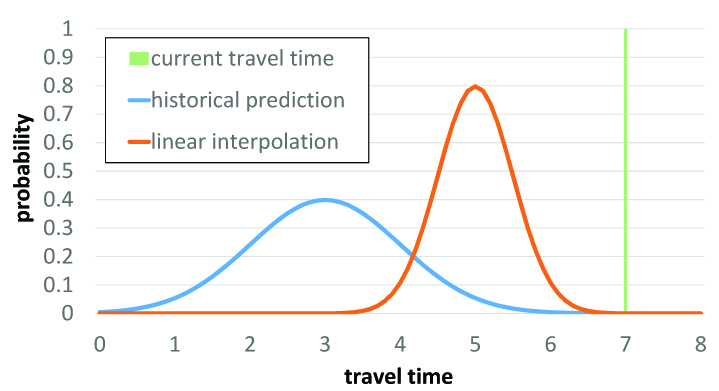
\includegraphics[width=0.80\columnwidth]{figures/tt_interpolation.jpg}
    \caption{Linear interpolation of ltt}
    \label{fig:interpolation}
\end{figure}

In the discrete case we adapt this concept and
obtain the following parameters.

\begin{gather}
F_{ij}^t(b) = \frac{1}{|H'|}\sum_{h\in H'} I(\lceil\frac{t - t_c}{\tau} \cdot 
c_{ij}^h + (1-\frac{t - t_c}{\tau})\cdot c_{i,j}^{t_c}\rceil^\phi = b)
\end{gather}

where $\lceil x \rceil^\phi$ rounds $x$ up to the next multiple of $\phi$ and
$I()$ is 1 whenever the corresponding statement is true.

\subsubsection{Prediction through Similar Historical Data}
\label{subsec:SH}
The third approach we propose is based on the idea that the current situation
is a crucial indicator on how the travel time of a street segment will develop
in the future. This approach thus further restricts the set $H'$, which is taken
into account for estimating the uncertain link travel time of the historical
approach. Specifically we only include times $h \in H'$ for estimating link travel time
$c_{i,j}^t$, for which $(i, j)$ had a similar link travel time at time
$h-(t-t_c)$ as the current link travel time $c_{i,j}^{t_c}$. We define
similarity in this context by a percentage threshold $\lambda$, which represents
the deviation from the current travel time.

 As an example, consider a street segment $(i, j)$ for which we want to
 predict the link travel time $c_{i,j}^{Tue, 9:20am}$ at 9:20am with the current
 time $t_c$ being Tue, 9:00am and the link travel time $c_{i,j}^{t_c} = 3$
 minutes. The parameter $\lambda$ is set to 10\%. Now the set $H'$ is defined by all times
that correspond to tuesdays 9:20am in the past year where the link travel time 20 minutes prior has been 3 minutes $\pm 18 sec$. Formally
$$H' = \{h|h = Tue,9:20am \wedge 162 sec \leq c_{i,j}^{Tue, 9:00am} \leq 198
sec\}$$

The value of $\lambda$ is obviously affecting the prediction result.
Setting $\lambda$ too small might result in not enough sample points in order to
obtain a meaningful uncertain prediction. On the other side setting $\lambda$
too large yields the historical prediction approach.


